
\begin{figure}[H]
    \centering
    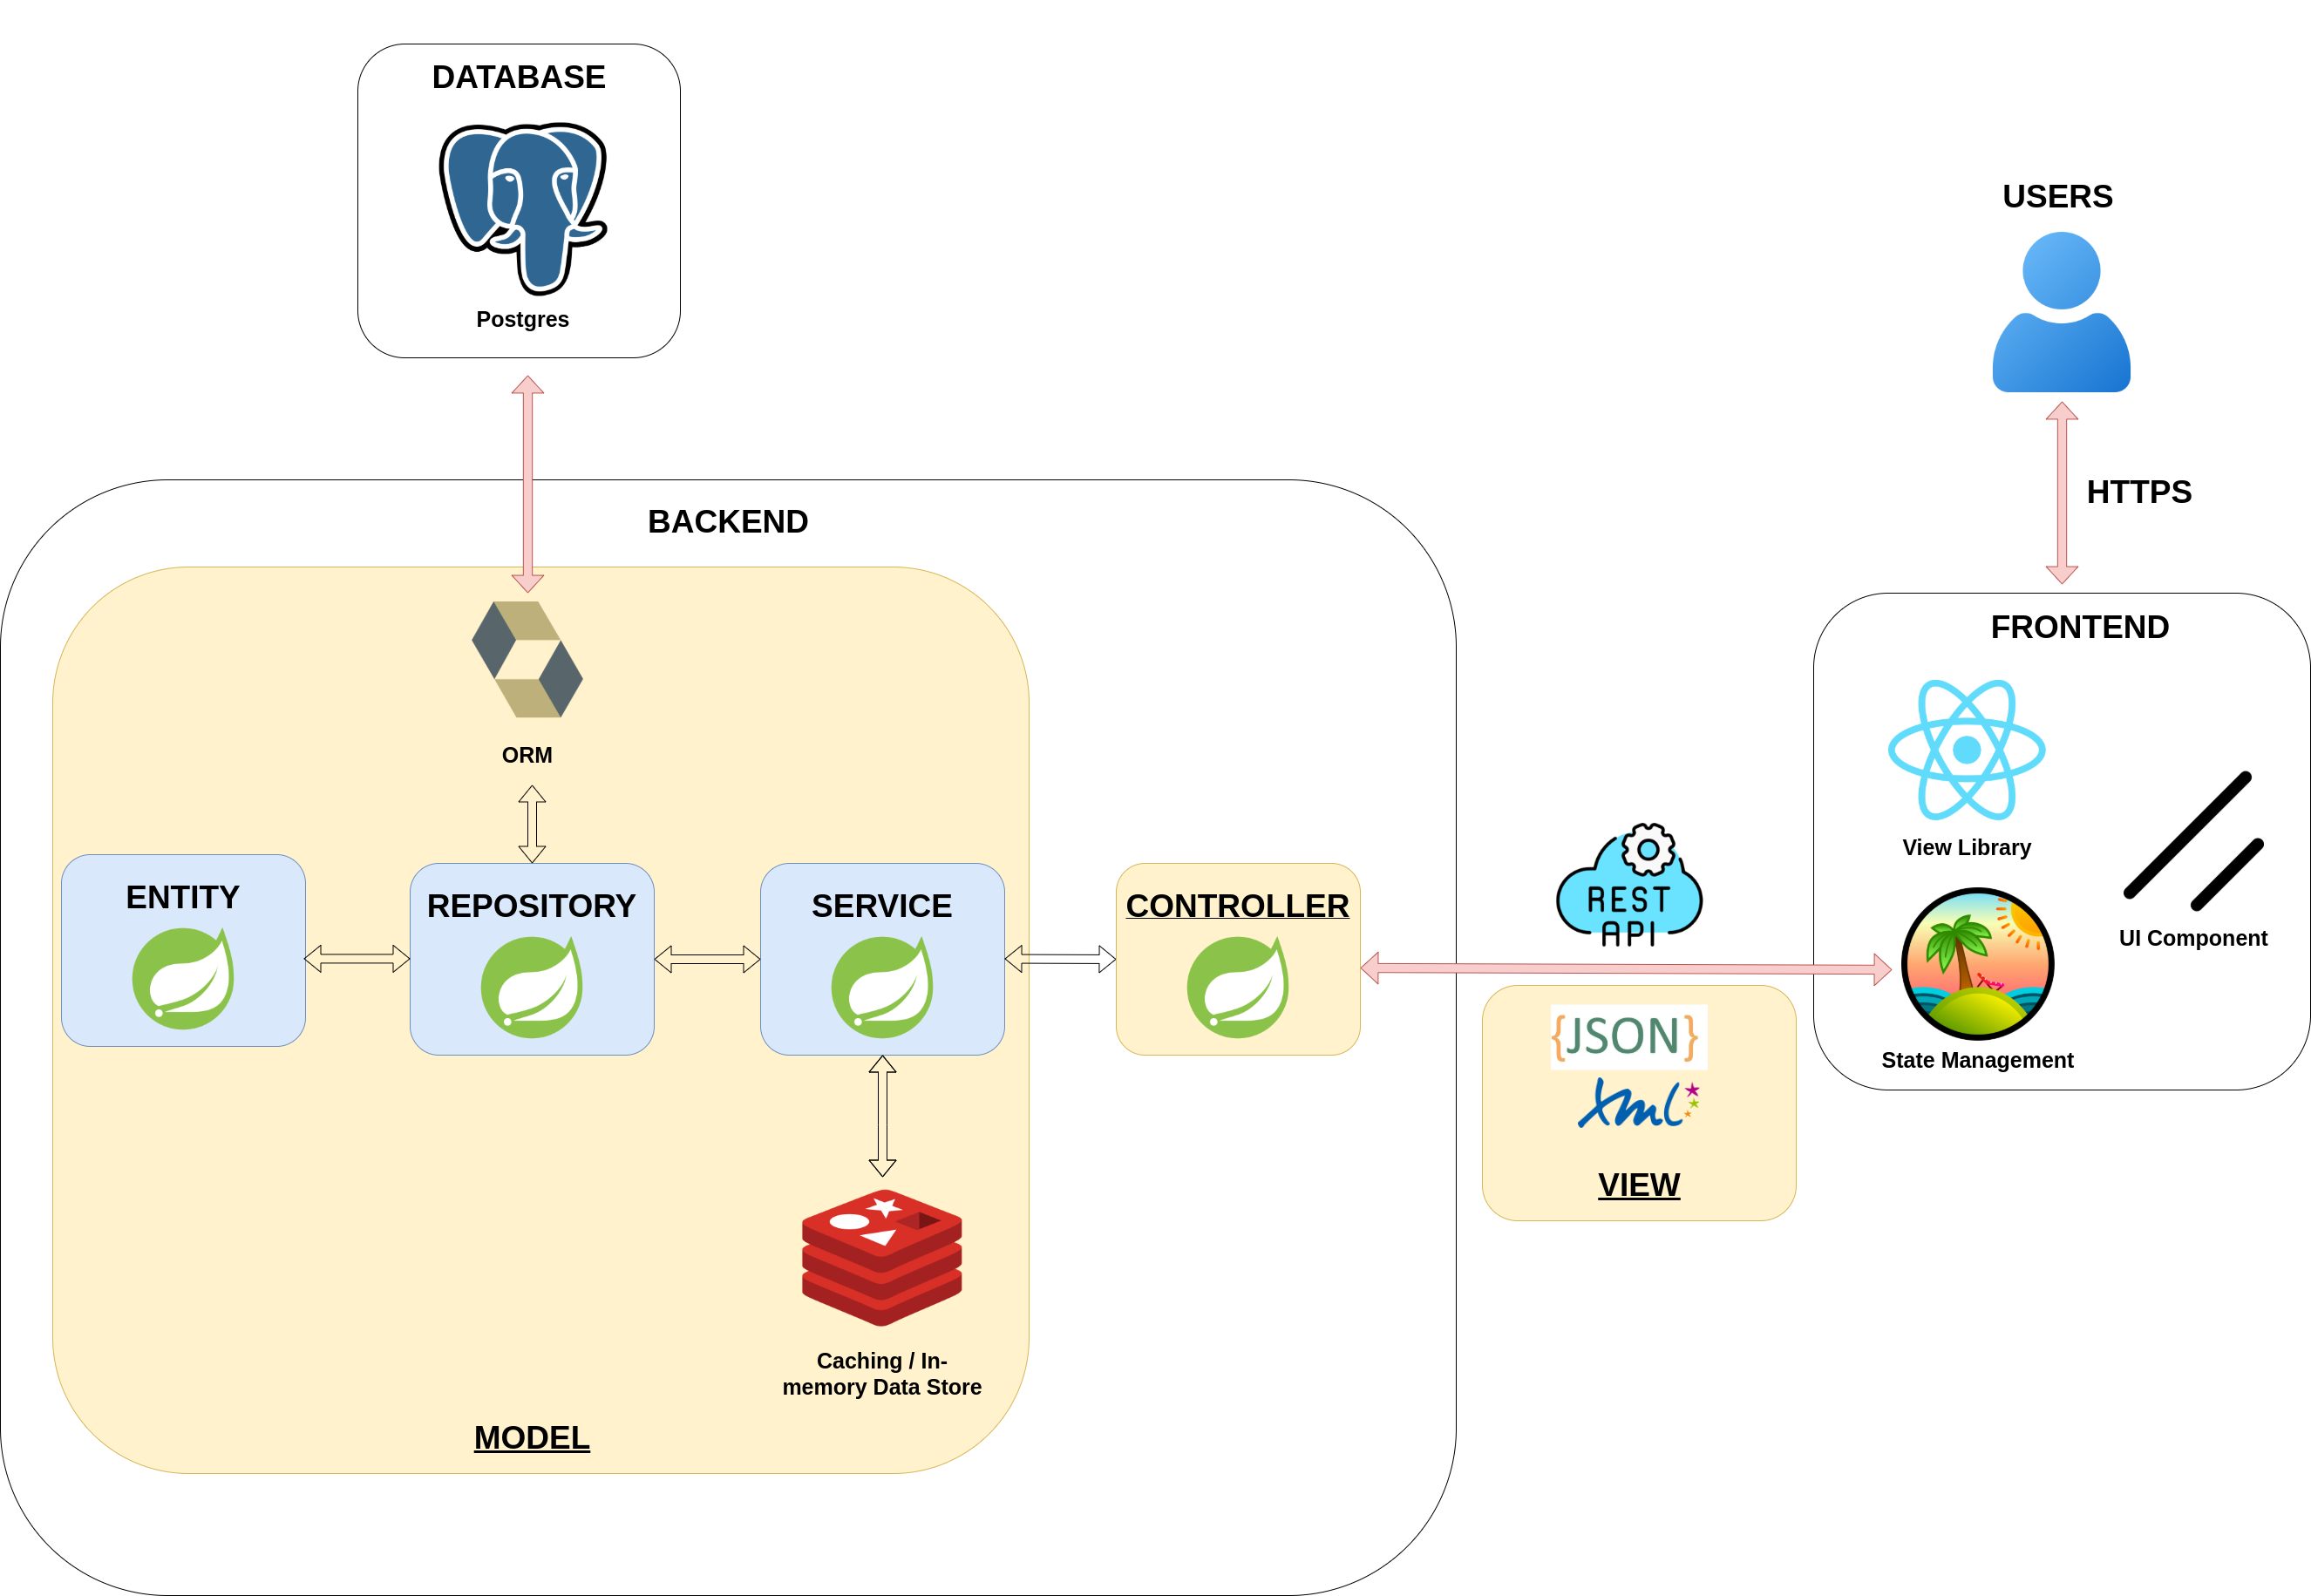
\includegraphics[width=10cm]{Images/kien-truc-he-thong.drawio.png}
    \vspace{0.5cm}
    \caption{Kiến trúc hệ thống}
    \label{fig:my_label}
\end{figure}

% Describing the importance of system architecture
Kiến trúc hệ thống đóng vai trò quan trọng trong dự án hệ thống quản lý nhà hàng. Nó xác định các thành phần chính của hệ thống và cách chúng tương tác với nhau để đáp ứng yêu cầu của người dùng. Kiến trúc này đảm bảo sự phân tách rõ ràng và sắp xếp logic giữa các thành phần, giúp dễ dàng quản lý, nâng cấp, mở rộng, tích hợp và tương tác giữa các thành phần khác nhau. Đồng thời, nó cung cấp khả năng mở rộng linh hoạt và thay đổi trong tương lai.

% Describing the architecture flow of the "Menu+" system
Dòng luồng kiến trúc của hệ thống "Menu+" được mô tả như sau:
\begin{itemize}
    \item Người dùng truy cập vào URL của hệ thống "Menu+" thông qua Internet.
    \item Khi truy cập, giao diện frontend của hệ thống được tải lên, bao gồm:
    \begin{itemize}
        \item Thư viện giao diện: ReactJS.
        \item Quản lý dữ liệu: TanStack.
        \item Thiết kế/Bố cục: ShadCN.
    \end{itemize}
    \item Nếu có hành động liên quan đến truy cập cơ sở dữ liệu hoặc dịch vụ bên thứ ba, hệ thống sử dụng TanStack để gửi yêu cầu đến server backend.
    \item Tại backend, Spring Boot Controller xử lý các yêu cầu API và ánh xạ chúng vào các URL tương ứng.
    \item Tiếp theo, tầng Service trong Spring Boot xác định hành động cần thực hiện dựa trên yêu cầu API.
    \item Nếu yêu cầu API cần truy cập cơ sở dữ liệu, Hibernate (ORM) sử dụng các entity để tạo truy vấn đến cơ sở dữ liệu PostgreSQL.
    \item Hibernate thực hiện truy vấn đến PostgreSQL, nơi lưu trữ dữ liệu của hệ thống.
    \item Để tối ưu hiệu suất, Service kiểm tra dữ liệu trong Redis (Caching/In-memory Data Store) trước; nếu không có, hệ thống truy vấn PostgreSQL và lưu kết quả vào Redis.
    \item Cuối cùng, Controller trả về kết quả dưới dạng JSON thông qua giao thức REST về frontend, và frontend hiển thị kết quả cho người dùng thông qua các UI Component.
\end{itemize}

% Describing how the system applies the MVC model with REST
Hệ thống "Menu+" áp dụng mô hình MVC (Model-View-Controller) kết hợp với REST API như sau:
\begin{itemize}
    \item \textbf{Model}: Bao gồm các thành phần liên quan đến dữ liệu và logic nghiệp vụ:
    \begin{itemize}
        \item \textit{Entity}: Định nghĩa cấu trúc dữ liệu (ví dụ: bảng Menu, Order) và ánh xạ với cơ sở dữ liệu PostgreSQL thông qua Hibernate.
        \item \textit{Service}: Chứa logic nghiệp vụ, xử lý các quy tắc kinh doanh (ví dụ: tính tổng hóa đơn, kiểm tra trạng thái món ăn).
        \item \textit{Caching}: Sử dụng Redis để lưu trữ dữ liệu truy cập thường xuyên, tối ưu hóa hiệu suất.
    \end{itemize}
    \item \textbf{Controller}: Được triển khai bởi Spring Boot Controller, chịu trách nhiệm xử lý các yêu cầu HTTP (GET, POST, PUT, DELETE) từ frontend, gọi đến Service để xử lý logic, và trả về phản hồi dưới dạng JSON qua REST API.
    \item \textbf{View}: Trong REST, View không phải là giao diện trực tiếp mà là dữ liệu JSON được trả về từ Controller. Frontend (ReactJS, TanStack, ShadCN) nhận dữ liệu này và hiển thị giao diện người dùng thông qua các UI Component.
\end{itemize}

% Concluding the architecture description
Kiến trúc này không chỉ đảm bảo sự phân tách rõ ràng giữa các tầng mà còn tận dụng REST API để giao tiếp hiệu quả giữa backend và frontend, đồng thời áp dụng MVC để tổ chức mã nguồn một cách logic và dễ bảo trì. \\

\begin{figure}[H]
    \centering
    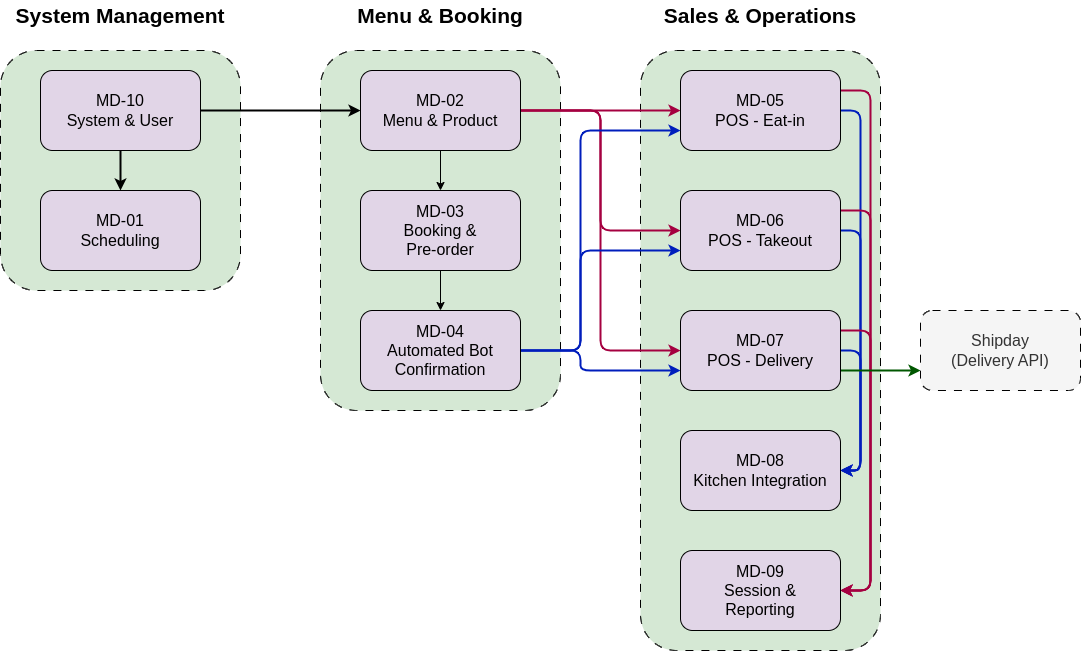
\includegraphics[width=10cm]{Images/kthtm.png}
    \vspace{0.5cm}
    \caption{Sơ đồ luồng kiến trúc hệ thống theo module chức năng}
    \label{fig:my_label}
\end{figure}

Sơ đồ luồng kiến trúc hệ thống được thiết kế để minh họa mối quan hệ và luồng dữ liệu giữa các module chức năng trong hệ thống quản lý nhà hàng. Các module được chia thành ba nhóm chính: Quản lý hệ thống (System Management), Quản lý thực thực đơn và đặt chỗ (Menu & Booking), và Bán hàng & Vận hành (Sales & Operations). Mỗi module, từ quản lý lịch làm việc (MD-01) đến báo cáo doanh thu (MD-09), được kết nối với nhau thông qua các luồng dữ liệu rõ ràng, hỗ trợ các chức năng như đặt chỗ, bán hàng tại chỗ, giao hàng và tích hợp với hệ thống bên ngoài như Shipday. Sơ đồ sử dụng bố cục lưới với các đường dẫn cong để đảm bảo tính trực quan và dễ theo dõi.

% Hệ thống bao gồm các thành phần như sau:
% \begin{enumerate}
%     \item \textbf{Frontend}
%     \begin{itemize}
%         \item Được phát triển bằng ReactJS.
%         \item Giao tiếp với backend thông qua RESTful API.
%         \item Cung cấp giao diện người dùng trực quan, tối ưu trải nghiệm (UX/UI), hỗ trợ responsive trên nhiều thiết bị.
%         \item Xử lý logic hiển thị, xác thực người dùng và tương tác với API.
%     \end{itemize}
%     \item \textbf{Backend}
%     \begin{itemize}
%         \item Được xây dựng bằng Spring Boot, theo mô hình Modular Monolithic và tổ chức theo nguyên tắc Domain-Driven Design (DDD).
%         \item Cung cấp API RESTful để frontend và các hệ thống khác có thể truy cập dữ liệu.
%         \item Xử lý các nghiệp vụ cốt lõi của hệ thống, bao gồm quản lý đặt bàn, thực đơn, đơn hàng, thanh toán, báo cáo, v.v.
%         \item Sử dụng Spring Security để xác thực và phân quyền người dùng.
%         \item Hỗ trợ caching bằng Redis để tăng hiệu suất truy vấn dữ liệu.
%     \end{itemize}
%     \item \textbf{Cơ sở dữ liệu}
%     \begin{itemize}
%         \item Sử dụng PostgreSQL làm hệ quản trị cơ sở dữ liệu chính.
%         \item Được thiết kế theo nguyên tắc CQRS (Command Query Responsibility Segregation) nhằm tối ưu hóa hiệu suất đọc/ghi.
%     \end{itemize}
%     \item \textbf{Third-party Integrations}
%     \begin{itemize}
%         \item Hỗ trợ kết nối với các cổng thanh toán như VNPay, Momo, Stripe để xử lý giao dịch.
%         \item Tích hợp với các dịch vụ bên ngoài như SMS, Email (SendGrid, Twilio), CRM, POS để mở rộng chức năng của hệ thống.
%     \end{itemize}

